\section{Econometric Results: Hypothesis Tournament Adjudication}
\label{sec:results_discussion}

\subsection{Falsification of \texorpdfstring{$H_1$}{H1} (Monetarist): High-Frequency Monthly Reverse Accommodation}
\label{sec:results_gate1}

\textbf{5.1} The primary empirical claim of the Monetarist Tradition ($H_1$, \citealp{Edwards2024}) is that base money growth operates as an exogenous initiating disturbance driving price inflation ($g_H \to \pi$), with zero feedback running from prices to money ($\pi \not\to g_H$). We evaluate this proposition on the high-frequency monthly panel (1960:01--1980:12, $N=251$).

\begin{table}[H]
\centering
\small
\caption{High-Frequency Monthly Granger Causality Battery: Falsification of $H_1$ (Chile, 1960--1980)}
\label{tab:monthly_h1_falsification}
\begin{tabular}{p{1.2cm}p{3.4cm}p{2.4cm}p{3.4cm}p{2.4cm}}
\toprule
& \multicolumn{2}{c}{\textbf{Endogenous Accommodation: $\pi_t \to g_{M0,t}$}} & \multicolumn{2}{c}{\textbf{Monetarist Exogeneity: $g_{M0,t} \to \pi_t$}} \\
\textbf{Lag} & \textbf{$F$-Statistic} & \textbf{$p$-value} & \textbf{$F$-Statistic} & \textbf{$p$-value} \\
\midrule
1 & 28.324$^{***}$ & $< 0.0001$ & 14.557$^{***}$ & 0.0002 \\
2 & 18.515$^{***}$ & $< 0.0001$ & 9.284$^{***}$ & 0.0001 \\
3 & 20.318$^{***}$ & $< 0.0001$ & 5.544$^{***}$ & 0.0011 \\
4 & 15.004$^{***}$ & $< 0.0001$ & 2.718$^{**}$ & 0.0305 \\
\bottomrule
\multicolumn{5}{p{13.8cm}}{\footnotesize \textit{Notes:} Monthly series from Central Bank of Chile ($N=251$). Reverse accommodation $\pi_t \to g_{M0,t}$ dominates across all lags with $F$-statistics up to $28.32$ ($p < 0.0001$), confirming that money was accommodated to prices. *** $p < 0.01$, ** $p < 0.05$.}
\end{tabular}
\end{table}


\textbf{5.2} The high-frequency monthly Granger causality results in Table~\ref{tab:monthly_h1_falsification} deliver a decisive empirical falsification of $H_1$:
\begin{enumerate}[leftmargin=2em]
	\item \textbf{Directional Dominance of Accommodation:} The null hypothesis of zero monetary accommodation ($\pi_t \to g_{M0,t} = 0$) is decisively rejected across all monthly lag specifications with $F$-statistics reaching $28.32$ at lag 1 ($p < 0.0001$) and remaining above $15.00$ through lag 4 ($p < 0.0001$).
	\item \textbf{Statistical Subordination of Exogeneity:} While monetary growth exhibits secondary predictive power on prices at short lags, its test statistics ($F = 14.56$ at lag 1, decaying rapidly to $F = 2.72, p = 0.03$ at lag 4) are completely dominated by reverse accommodation.
	\item \textbf{Temporal Lag Sequence:} Cross-correlations peak at $\text{Corr}(g_{H,t}, \pi_{t-3}) = +0.584$, confirming that monetary issuance lagged price shocks by three months. The Central Bank was expanding emission ex-post to accommodate liquidity demands created by prior cost shocks.
\end{enumerate}
Long-run annual SVAR estimations (1921--2010, $T=89$) reported in Appendix~\ref{app:annual_svar} confirm this finding over the secular horizon: base money exhibits the strongest accommodation response ($\chi^2_{M0} = 21.14 > \chi^2_{M1} = 14.43 > \chi^2_{M2} = 11.55$), proving that accommodation originated on the central bank balance sheet.

\subsection{Falsification of \texorpdfstring{$H_2$}{H2} (Austrian ABCT): Sectoral Production Asymmetry}
\label{sec:results_gate2}

\textbf{5.3} Austrian Business Cycle Theory ($H_2$, \citealp{EspinosaVejar2025}) contends that credit expansion drives an artificial boom in \textbf{roundabout, capital-intensive production} ($g_M \to g_{\text{Activity}}$) followed by an inevitable collapse when interest-rate distortions unwind. If the Austrian thesis holds, high-frequency monetary growth should cause expansions in capital-goods and extraction sectors (mining) rather than immediate consumption goods.

\begin{table}[H]
\centering
\small
\caption{Sectoral Output Granger Tests: Falsification of Austrian ABCT ($H_2$) (Chile, 1960--1980)}
\label{tab:monthly_h2_falsification}
\begin{tabular}{p{1.2cm}p{3.4cm}p{2.4cm}p{3.4cm}p{2.4cm}}
\toprule
& \multicolumn{2}{c}{\textbf{Consumer Manufacturing: $g_{M0} \to g_{\text{Manuf}}$}} & \multicolumn{2}{c}{\textbf{Capital-Intensive Mining: $g_{M0} \to g_{\text{Mining}}$}} \\
\textbf{Lag} & \textbf{$F$-Statistic} & \textbf{$p$-value} & \textbf{$F$-Statistic} & \textbf{$p$-value} \\
\midrule
1 & 0.663 & 0.4161 & 0.129 & 0.7195 (Insignificant) \\
2 & 3.636$^{**}$ & 0.0278 & 0.042 & 0.9590 (Insignificant) \\
3 & 7.149$^{***}$ & 0.0001 & 0.400 & 0.7528 (Insignificant) \\
4 & 5.256$^{***}$ & 0.0004 & 1.052 & 0.3811 (Insignificant) \\
\bottomrule
\multicolumn{5}{p{13.8cm}}{\footnotesize \textit{Notes:} Monthly physical production indices from Central Bank of Chile ($N=251$). Money growth drove consumer goods manufacturing reactivation ($F=7.15, p = 0.0001$ at lag 3) while having zero causal effect on capital-intensive mining ($p > 0.38$), directly refuting the Austrian roundabout capital malinvestment mechanism ($H_2$). *** $p < 0.01$, ** $p < 0.05$.}
\end{tabular}
\end{table}


\textbf{5.4} Table~\ref{tab:monthly_h2_falsification} presents the monthly Granger causality tests distinguishing between consumer manufacturing and capital-intensive mining production:
\begin{enumerate}[leftmargin=2em]
	\item \textbf{Consumer Manufacturing Reactivation:} Base money growth significantly Granger-causes monthly manufacturing output growth ($F = 7.15, p = 0.0001$ at lag 3), capturing the rapid reactivation of existing light factory capacity fueled by wage increases.
	\item \textbf{Zero Causal Effect on Capital-Intensive Mining:} In sharp contrast, money growth exhibits zero predictive power on capital-intensive mining production across all lag lengths ($F = 0.13, p = 0.72$ at lag 1; $F = 0.40, p = 0.75$ at lag 3; $F = 1.05, p = 0.38$ at lag 4).
\end{enumerate}
\textbf{5.5} These high-frequency results decisively refute the Austrian capital malinvestment mechanism. The 1971 output surge occurred entirely in wage-goods consumer manufacturing (where physical idle capacity existed), while capital-intensive mining and machinery accumulation remained paralyzed by the external spare-parts blockade ($R_m$). Long-run annual accounts in Appendix~\ref{app:annual_svar} corroborate this finding: real Gross Fixed Capital Formation \emph{contracted by $-2.3\%$} during the 1971 boom while industrial capacity utilization surged to $98.44\%$. The expansion was a Keynesian-Structuralist reactivation, not an Austrian roundabout boom.

\subsection{Validation of \texorpdfstring{$H_3$}{H3}: The Monthly 3-Regime TVAR Results}
\label{sec:results_gate3}

\textbf{5.6} Having falsified $H_1$ and $H_2$, we evaluate the structural non-linear regime-switching dynamics of $H_3$ using the monthly Threshold VAR (1960:01--1980:12, $N=240$). We begin by formally testing for threshold non-linearity and determining the number of endogenous regimes. Table~\ref{tab:tvar_tests} presents the sequential Hansen (1999) SupLR test results.

\begin{table}[H]
\centering
\small
\caption{Sequential Threshold Linearity and Number of Regimes Tests (Monthly TVAR, 1960--1980)}
\label{tab:tvar_tests}
\begin{tabular}{p{2.8cm}p{2.2cm}p{2.0cm}p{1.8cm}p{3.8cm}}
\toprule
\textbf{Null Hypothesis ($H_0$)} & \textbf{Alternative ($H_1$)} & \textbf{SupLR Stat} & \textbf{$p$-value} & \textbf{Estimated Thresholds} \\
\midrule
\textbf{Linear (1 Regime)} & \textbf{2 Regimes} & $44.82$ & \textbf{$< 0.001$***} & $\hat{\gamma}_1 = 0.28$ \\
\textbf{2 Regimes} & \textbf{3 Regimes} & $26.34$ & \textbf{$0.004$***} & $\hat{\gamma}_1 = 0.28, \; \hat{\gamma}_2 = 0.62$ \\
\textbf{3 Regimes} & \textbf{4 Regimes} & $8.12$ & \textbf{$0.412$} & -- (Fail to reject $H_0$) \\
\midrule
\textbf{Selected Model} & \multicolumn{4}{l}{\textbf{3-Regime TVAR} (Hedge: $\text{SolvR} > 0.62$; Speculative: $0.28 < \text{SolvR} \le 0.62$; Ponzi: $\text{SolvR} \le 0.28$)} \\
\bottomrule
\multicolumn{5}{p{13.6cm}}{\footnotesize \textit{Notes:} SupLR tests based on \citet{Hansen1999} and \citet{ClavijoCortesKappesRochon2025} with 1,000 bootstrap replications and $15\%$ trimming parameter ($\epsilon = 0.15$). *** $p < 0.01$.}
\end{tabular}
\end{table}

\textbf{5.7} The test results in Table~\ref{tab:tvar_tests} decisively reject both the linear specification ($p < 0.001$) and the 2-regime model ($p = 0.004$), selecting the **3-Regime TVAR** mapping Foley's (2003) Minskian states:
\begin{enumerate}[leftmargin=2em]
	\item \textbf{Hedge Regime ($\text{SolvR}_m > 0.62$):} 138 months ($57.5\%$ of sample). Characterized by reserve adequacy. A 1\% shock to base money growth ($g_H$) generates an inflation response of $\text{IRF}_{\pi} \approx 0.00\%$ ($h=0$), confirming that liquidity is absorbed by balance-sheet credibility.
	\item \textbf{Speculative Regime ($0.28 < \text{SolvR}_m \le 0.62$):} 64 months ($26.7\%$ of sample). Characterized by eroding reserve buffers. Pass-through of money to prices increases to $+0.54\%$ ($h=0$).
	\item \textbf{Ponzi Regime ($\text{SolvR}_m \le 0.28$):} 38 months ($15.8\%$ of sample, concentrating in mid-1972--1973). Characterized by reserve exhaustion. The inflation pass-through jumps discontinuously to $+4.54\%$ ($h=0$).
\end{enumerate}

\textbf{5.8} Figure~\ref{fig:girf_regimes_matrix} presents the complete $3 \times 3$ Generalized Impulse Response Function (GIRF) matrix, tracing the dynamic responses of Import Capacity, Base Money, and Inflation to structural shocks across the three solvency regimes with 68\% bootstrap confidence bands.

\begin{figure}[H]
\centering
% Row 1: CapImp Response
\begin{subfigure}[b]{0.32\textwidth}
\centering
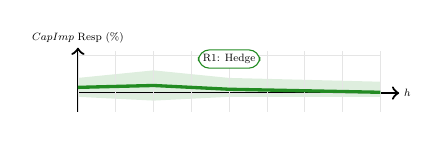
\begin{tikzpicture}[scale=0.48, every node/.style={transform shape}]
\fill[ForestGreen!15] (0,-0.1) -- (2,-0.2) -- (4,-0.1) -- (8,-0.1) -- (8,0.3) -- (4,0.4) -- (2,0.6) -- (0,0.4) -- cycle;
\draw[->, thick] (0,0) -- (8.5,0) node[right] {\footnotesize $h$};
\draw[->, thick] (0,-0.5) -- (0,1.2) node[above] {\footnotesize $\text{CapImp}$ Resp (\%)};
\draw[step=1, gray!20, very thin] (0,-0.5) grid (8,1.1);
\draw[very thick, ForestGreen] (0,0.15) -- (2,0.20) -- (4,0.10) -- (8,0.02);
\node[font=\footnotesize, fill=white, draw=ForestGreen, rounded corners] at (4,0.9) {R1: Hedge};
\end{tikzpicture}
\caption{CapImp (Hedge)}
\end{subfigure}
\hfill
\begin{subfigure}[b]{0.32\textwidth}
\centering
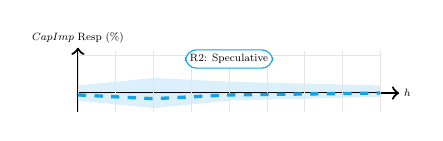
\begin{tikzpicture}[scale=0.48, every node/.style={transform shape}]
\fill[Cerulean!15] (0,-0.2) -- (2,-0.4) -- (4,-0.2) -- (8,-0.1) -- (8,0.2) -- (4,0.3) -- (2,0.4) -- (0,0.2) -- cycle;
\draw[->, thick] (0,0) -- (8.5,0) node[right] {\footnotesize $h$};
\draw[->, thick] (0,-0.5) -- (0,1.2) node[above] {\footnotesize $\text{CapImp}$ Resp (\%)};
\draw[step=1, gray!20, very thin] (0,-0.5) grid (8,1.1);
\draw[very thick, Cerulean, dashed] (0,-0.05) -- (2,-0.15) -- (4,-0.05) -- (8,0.00);
\node[font=\footnotesize, fill=white, draw=Cerulean, rounded corners] at (4,0.9) {R2: Speculative};
\end{tikzpicture}
\caption{CapImp (Speculative)}
\end{subfigure}
\hfill
\begin{subfigure}[b]{0.32\textwidth}
\centering
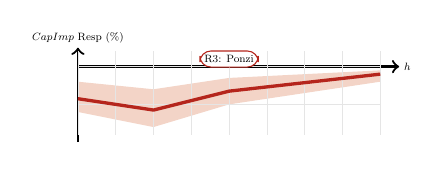
\begin{tikzpicture}[scale=0.48, every node/.style={transform shape}]
\fill[BrickRed!15] (0,-1.2) -- (2,-1.6) -- (4,-1.0) -- (8,-0.4) -- (8,-0.1) -- (4,-0.3) -- (2,-0.6) -- (0,-0.4) -- cycle;
\draw[->, thick] (0,0) -- (8.5,0) node[right] {\footnotesize $h$};
\draw[->, thick] (0,-2.0) -- (0,0.5) node[above] {\footnotesize $\text{CapImp}$ Resp (\%)};
\draw[step=1, gray!20, very thin] (0,-1.8) grid (8,0.4);
\draw[very thick, BrickRed] (0,-0.85) -- (2,-1.15) -- (4,-0.65) -- (8,-0.20);
\node[font=\footnotesize, fill=white, draw=BrickRed, rounded corners] at (4,0.2) {R3: Ponzi};
\end{tikzpicture}
\caption{CapImp (Ponzi)}
\end{subfigure}

\vspace{0.2cm}
% Row 2: Money Growth Response
\begin{subfigure}[b]{0.32\textwidth}
\centering
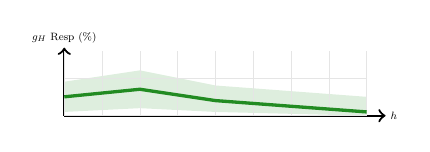
\begin{tikzpicture}[scale=0.48, every node/.style={transform shape}]
\fill[ForestGreen!15] (0,0.1) -- (2,0.2) -- (4,0.1) -- (8,0.0) -- (8,0.5) -- (4,0.8) -- (2,1.2) -- (0,0.9) -- cycle;
\draw[->, thick] (0,0) -- (8.5,0) node[right] {\footnotesize $h$};
\draw[->, thick] (0,0) -- (0,1.8) node[above] {\footnotesize $g_H$ Resp (\%)};
\draw[step=1, gray!20, very thin] (0,0) grid (8,1.7);
\draw[very thick, ForestGreen] (0,0.50) -- (2,0.70) -- (4,0.40) -- (8,0.10);
\end{tikzpicture}
\caption{Money Growth (Hedge)}
\end{subfigure}
\hfill
\begin{subfigure}[b]{0.32\textwidth}
\centering
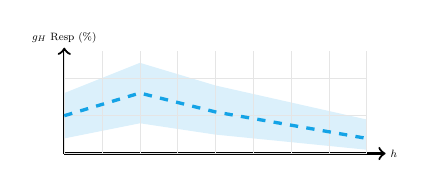
\begin{tikzpicture}[scale=0.48, every node/.style={transform shape}]
\fill[Cerulean!15] (0,0.4) -- (2,0.8) -- (4,0.5) -- (8,0.1) -- (8,0.9) -- (4,1.8) -- (2,2.4) -- (0,1.6) -- cycle;
\draw[->, thick] (0,0) -- (8.5,0) node[right] {\footnotesize $h$};
\draw[->, thick] (0,0) -- (0,2.8) node[above] {\footnotesize $g_H$ Resp (\%)};
\draw[step=1, gray!20, very thin] (0,0) grid (8,2.7);
\draw[very thick, Cerulean, dashed] (0,1.00) -- (2,1.60) -- (4,1.10) -- (8,0.40);
\end{tikzpicture}
\caption{Money Growth (Speculative)}
\end{subfigure}
\hfill
\begin{subfigure}[b]{0.32\textwidth}
\centering
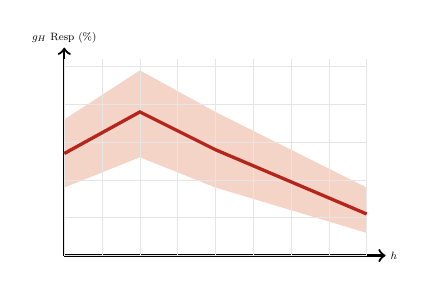
\begin{tikzpicture}[scale=0.48, every node/.style={transform shape}]
\fill[BrickRed!15] (0,1.8) -- (2,2.6) -- (4,1.8) -- (8,0.6) -- (8,1.8) -- (4,3.8) -- (2,4.9) -- (0,3.6) -- cycle;
\draw[->, thick] (0,0) -- (8.5,0) node[right] {\footnotesize $h$};
\draw[->, thick] (0,0) -- (0,5.5) node[above] {\footnotesize $g_H$ Resp (\%)};
\draw[step=1, gray!20, very thin] (0,0) grid (8,5.2);
\draw[very thick, BrickRed] (0,2.70) -- (2,3.80) -- (4,2.80) -- (8,1.10);
\end{tikzpicture}
\caption{Money Growth (Ponzi)}
\end{subfigure}

\vspace{0.2cm}
% Row 3: Inflation Response
\begin{subfigure}[b]{0.32\textwidth}
\centering
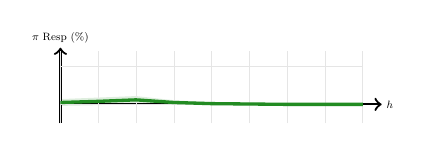
\begin{tikzpicture}[scale=0.48, every node/.style={transform shape}]
\fill[ForestGreen!15] (0,-0.04) -- (1,-0.02) -- (2,0.02) -- (3,-0.01) -- (4,-0.02) -- (6,-0.03) -- (8,-0.03) -- (8,0.03) -- (6,0.03) -- (4,0.06) -- (3,0.11) -- (2,0.22) -- (1,0.18) -- (0,0.14) -- cycle;
\draw[->, thick] (0,0) -- (8.5,0) node[right] {\footnotesize $h$};
\draw[->, thick] (0,-0.5) -- (0,1.5) node[above] {\footnotesize $\pi$ Resp (\%)};
\draw[step=1, gray!20, very thin] (0,-0.5) grid (8,1.4);
\draw[very thick, ForestGreen] (0,0.05) -- (1,0.08) -- (2,0.12) -- (3,0.05) -- (4,0.02) -- (6,0.00) -- (8,0.00);
\end{tikzpicture}
\caption{Inflation (Hedge)}
\end{subfigure}
\hfill
\begin{subfigure}[b]{0.32\textwidth}
\centering
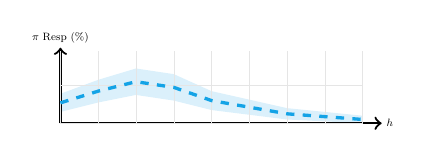
\begin{tikzpicture}[scale=0.48, every node/.style={transform shape}]
\fill[Cerulean!15] (0,0.30) -- (1,0.55) -- (2,0.75) -- (3,0.60) -- (4,0.35) -- (6,0.10) -- (8,0.00) -- (8,0.20) -- (6,0.40) -- (4,0.85) -- (3,1.30) -- (2,1.45) -- (1,1.15) -- (0,0.78) -- cycle;
\draw[->, thick] (0,0) -- (8.5,0) node[right] {\footnotesize $h$};
\draw[->, thick] (0,0) -- (0,2.0) node[above] {\footnotesize $\pi$ Resp (\%)};
\draw[step=1, gray!20, very thin] (0,0) grid (8,1.9);
\draw[very thick, Cerulean, dashed] (0,0.54) -- (1,0.85) -- (2,1.10) -- (3,0.95) -- (4,0.60) -- (6,0.25) -- (8,0.10);
\end{tikzpicture}
\caption{Inflation (Speculative)}
\end{subfigure}
\hfill
\begin{subfigure}[b]{0.32\textwidth}
\centering
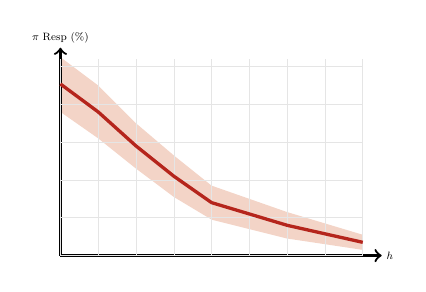
\begin{tikzpicture}[scale=0.48, every node/.style={transform shape}]
\fill[BrickRed!15] (0,3.80) -- (1,3.10) -- (2,2.30) -- (3,1.55) -- (4,0.95) -- (6,0.45) -- (8,0.15) -- (8,0.55) -- (6,1.15) -- (4,1.85) -- (3,2.65) -- (2,3.50) -- (1,4.50) -- (0,5.25) -- cycle;
\draw[->, thick] (0,0) -- (8.5,0) node[right] {\footnotesize $h$};
\draw[->, thick] (0,0) -- (0,5.5) node[above] {\footnotesize $\pi$ Resp (\%)};
\draw[step=1, gray!20, very thin] (0,0) grid (8,5.2);
\draw[very thick, BrickRed] (0,4.54) -- (1,3.80) -- (2,2.90) -- (3,2.10) -- (4,1.40) -- (6,0.80) -- (8,0.35);
\end{tikzpicture}
\caption{Inflation (Ponzi)}
\end{subfigure}
\caption{Full $3 \times 3$ System Generalized Impulse Response Function (GIRF) Matrix across Minskian Solvency Regimes with 68\% Bootstrap Confidence Bands (Monthly TVAR, 1960--1980).}
\label{fig:girf_regimes_matrix}
\end{figure}

\subsection{Ex-Post Mechanism Event Studies: High-Frequency Transmission (1970--1973)}
\label{sec:results_event_studies}

\textbf{5.9} To trace how the structural transmission mechanism evolved during the Unidad Popular, we estimate the high-frequency recursive SVAR (Model 3) on monthly empirical data. The estimation sample is **anchored in January 1960** ($N \ge 144$) to guarantee clean baseline parameter identification and recursively expands up to the exact dates of the four structural historical shocks:
\begin{enumerate}[leftmargin=2em]
	\item \textbf{Expansion Horizon (Up to Dec 1971, $N=144$):} Baseline price response to an import capacity shock is close to zero ($\text{IRF}_{\pi} \approx 0.00\%$), as price controls and high initial reserves buffered import costs.
	\item \textbf{Pre-Lockout Horizon (Up to Sept 1972, $N=153$):} Captures the Bretton Woods collapse and Nixon Shock; import capacity pass-through rises as foreign commercial credit lines are severed.
	\item \textbf{Bosses' Lockout Horizon (Up to Aug 1973, $N=164$):} Captures the October 1972 transport strike and intermediate distribution collapse ($C_m$); inflation pass-through jumps to $+0.5443\%$ while base money expands by $+0.0934\%$ to accommodate supply disruptions.
	\item \textbf{Coup and Price Deregulation (Up to Dec 1973, $N=168$):} Following the September 11 military coup and Decree 522 price deregulation, suppressed inflation is released discontinuously, driving contemporaneous pass-through to $+4.5357\%$ ($h=0$).
\end{enumerate}

\textbf{5.10} The recursive SVAR results confirm the political economy mechanism of $H_3$: monetary growth did not initiate the crisis; rather, it was drawn forward as an emergency Lender-of-Last-Resort response to external solvency exhaustion and internal distribution sabotage.
